\section{Frozen predictions: the full record}\label{app:frozen}

This appendix gives every prediction frozen for the later tests (Tables~\ref{tab:frozen} and~\ref{tab:frozen2}) with its source, its scoring rule and what it is blind to, and the outcomes in hand in detail; \S\ref{sec:frozen} summarizes them, \S\ref{sec:h200}, \S\ref{sec:rescue} and \S\ref{sec:basin} report the H200, rescue and basin outcomes, and Table~\ref{tab:timeline-r11} gives the GitHub push times. Each registered test has a FILLED registration committed and tagged before its first job, except that the Llama-3.1-8B registration (\texttt{1559f8e}) was pushed 47\,s before its jobs were submitted but not tagged. BASIN-1's reached GitHub at 20:04:30 CDT on 2026-10-30, 68 minutes before its jobs were submitted; R1's and R4's at 22:39:02, 22 minutes before theirs; and BASIN-2's, TOOLSLOW's and SHED's at 02:10:48 and 02:28:09 CDT on 2026-10-31, before their jobs were submitted at 04:21 (Table~\ref{tab:ledger}). Every outcome is reported against these rules, misses included.

\begin{figure*}[t]\centering
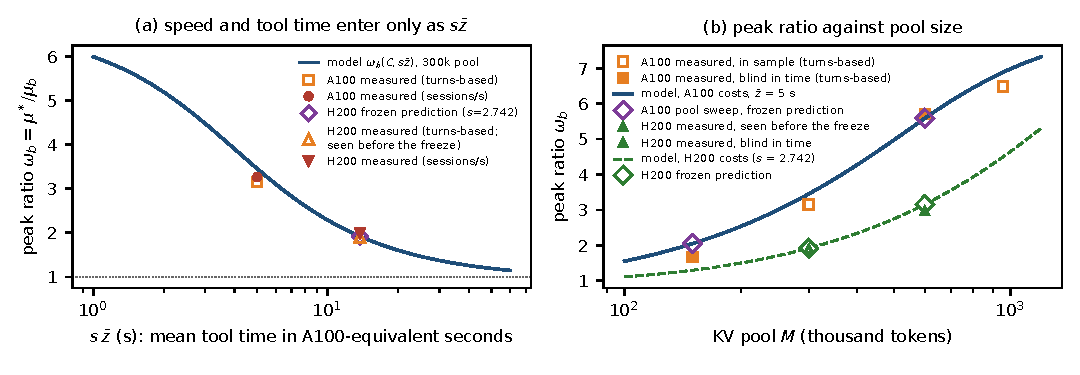
\includegraphics[width=\textwidth]{figs/fig9_theory_scaling.pdf}
\caption{Frozen predictions of the peak ratio $\omega_b=\mu^*/\mu_b$ (fluid model, in model units). (a) Against $s\bar z$, the mean tool time in A100-equivalent seconds, for the 300k pool (Proposition~\ref{prop:scaling}); squares and dot: the A100, measured (turns-based, sessions/s); diamond: the H200 prediction ($s=2.742$). (b) Against the pool size, A100 costs, $\bar z=5$\,s; squares: measured cells (turns-based); diamonds: the pool-sweep predictions. Triangles: the H200 measured peak ratio against its $\lref$, 1.89 turns-based and 1.99 in sessions/s (Table~\ref{tab:frozen}), values the first author had seen before the freeze. The pool-sweep outcomes are pending. Table~\ref{tab:frozen} quotes the primary predictions (F1, against $\lref$), which are lower than the plotted fluid values by 0.1\% (H200) to 8.6\% (150k).}\label{fig:fpscale}
\end{figure*}

\begin{table*}[tp]
\centering\footnotesize
\caption{Frozen predictions and their tests. Each prediction was committed under the tag named before any of its results was read by the agents that made it (for the H200 and BASIN-1 exceptions see their rows; the theory's fresh-seed probabilities were not declared for that test before it ran); scoring rules and tolerances were frozen with it (\fpath{notes/THEORY_r13_scoring.md} for the theory; the registration file or \fpath{configs/r11_*_predict.yaml} otherwise). ``Theory'': the model of \S\ref{sec:fp}, tag \texttt{r13-theory-pred} (\S\ref{sec:fp-val}), files under \fpath{results/theory/merged/}; ``pred2'': new drivers calling the same frozen model, tag \texttt{r13-theory-pred2} (commit \texttt{cfa7712}, pushed 04:20:20 CDT, before the first BASIN-2, TOOLSLOW or SHED job by its freeze record; files under \fpath{results/theory/pred2/} at that tag). ``Simulator'': the calibrated simulator of \S\ref{sec:sim}. $\omega_{\mathrm{ref}}=\mu^*/\lref$ (turns-based), with $\lref$ the cell's measured E0a rate (pool sweep: the A100 300k value, 0.0715\sps; H200 600k: the H200 300k value, 0.194\sps; Llama: the model's a priori $\lmiss$); hit is the fraction of all turns of a closed run that hit (first turns always miss, so at most 0.932), the Stage~C estimator; stuck means a hit fraction below 0.2 over the evaluation window.}\label{tab:frozen}
\setlength{\tabcolsep}{3pt}
\begin{tabular}{@{}>{\raggedright\arraybackslash}p{2.6cm} >{\raggedright\arraybackslash}p{7.3cm} >{\raggedright\arraybackslash}p{3.2cm} >{\raggedright\arraybackslash}p{3.8cm}@{}}
\toprule
Test & Frozen prediction & Source & Outcome\\
\midrule
H200 NVL, SGLang, 300k pool: curve & $\omega_{\mathrm{ref}}=1.92$ (band 1.65--1.92 over the five cost variants; fluid 1.66--1.96; A100: 3.27 predicted, 3.15 measured); all-miss onset $n_b=41.3$ (A100: 32.7); 0.5-hit crossing at $n=37.3\pm3$; hit 0.67 (F1) at the peak, $n\approx32.5$ (0.69 at $n=32$, the value the freeze record gives). Refuted if $\omega_{\mathrm{ref}}\ge2.4$, hit$(32)<0.5$ or hit$(48)\ge0.5$; the first two are not blind to the first author, who had seen $n\le32$. & theory, \fpath{h200_300k*.json}; $s=2.742$ fitted to the H200's all-miss token rate & Measured, not a registered test (window $(1,1.3)\,\lref$, too narrow for the registration rule): $\omega_{\mathrm{ref}}=1.89$ (sessions-based 1.99); peak at $n=32$; crossing $\approx38.9$ (38.8 on the nine-point curve); hit 0.74 at $n=32$, 0.22 at 48. No rule fires\\
\addlinespace[0.3pt]
H200: cliff bracket, $n=36$, 44, 52 & Hit, fluid: 0.56 at $n=36$ (variants 0.52--0.57), 0 at 44 and 52; F1: 0.53 (0.50--0.53), 0.08, 0.002 (from the frozen curves, not the freeze record). At the original points $n=40$ and 48: fluid 0.27 and 0, F1 0.28 and 0.01 & theory, \fpath{h200_300k*.json} (closed curve) & Hit 0.61, 0.32, 0.16 (crossing $\approx38.9$), and 0.46, 0.22 at $n=40$, 48: closest at 36; from 40 the tail is softer than predicted, so $n_b=41.3$ is early. Blind in time (36, 44, 52); by access only (40, 48)\\
\addlinespace[0.3pt]
H200: from-empty edge & F2 edge $1.39\,\lref$ (1.24--1.40 over the cost variants); scored on the original E0b runs 17168377--82, not the later reseeds & theory, \fpath{h200_300k*.json} & Stable at 1.3, unstable at 1.4 $\lref$ (nominal): edge in $[1.3,1.4)$, contains 1.39. Realized rates: ten runs monotone, edge 1.496--1.503, so F2 about 7\% pessimistic, as on the A100. Reseeds (post hoc): 1.3 stable in 3 of 3 seeds, 1.4 in 2 of 3 (F2 probability of staying stable: 0.72, 0.48). Original runs blind by access only\\
\addlinespace[0.3pt]
H200 NVL, 600k pool & pred2 (jobs submitted at 02:50--02:51 CDT, before its push, not eligible to start before 05:00; first start 05:27): $n_b=69.9$, as Proposition~\ref{prop:nb}(c) gives from the 600k A100 onset and $s$; $\omega_{\mathrm{ref}}=3.20$ (fluid 3.27); crossing 66.6; F2 edge $2.57\,\lref$ & pred2, \fpath{h200_600k.json} & \pending{Stage C 17169672--80, E0b 17169682--87}\\
\addlinespace[0.3pt]
Llama-3.1-8B, SGLang, A100, 300k & Theory, a priori: $M/E_S=27.8$ for any speed, $n_b=32.0$, crossing 30.9, $\omega_{\mathrm{ref}}=3.37$, edge $2.46\,\lmiss$; after the cell's $\lmiss$ is measured, every quantity comes from the frozen speed table. Refuted if the crossing lies outside the table's value $\pm3$, or $\mu(48)$ is within 10\% of the peak. Simulator, costs scaled to the measured all-miss rate: peak at $n=20$, $\omega_{\mathrm{ref}}=3.52$, crossing 30.6, edge $2.5\,\lmiss$, paired test passes at every candidate rate. & theory, \fpath{llama31_8b_300k*.json}; simulator, tag \texttt{r12-llama31-\allowbreak predictions-frozen}, \fpath{notes/PREDICTIONS_llama31.md} & Registered (\texttt{1559f8e}, pushed 07:49:15 CDT on 10-31; 1.35, 1.65 $\lref$, cap 20). \pending{Stage C 17166814--16, E0b 17169565--70, E2 17170409--26}\\
\addlinespace[0.3pt]
Pool sweep, SGLang, A100, 150k and 600k & $\omega_{\mathrm{ref}}=1.87$ and 5.47; $n_b=18.3$ and 61.2; crossing 16.9 and 60.0; F2 edge 1.09 and $4.53\,\lref$ (second criterion 1.47 and 4.82). Refuted if $\omega_{\mathrm{ref}}\ge2.5$ or hit$(24)\ge0.5$ at 150k, or $\omega_{\mathrm{ref}}<4.5$ or hit$(48)<0.5$ at 600k. No fitted parameter. & theory, \fpath{a100_pool150k.json}, \fpath{a100_pool600k.json} & \pending{Stage C 17168864--69, E0b 17168870--81}\\
\addlinespace[0.3pt]
Fresh-seed E0b, 300k, seeds 3--5, 2.0 and 2.5 $\lref$ & Simulator: stable in 3 of 3 at both rates, so the seed-0 bracket is not replicated. Theory (F2): unstable with probability 0.15 and 0.69 per seed. & simulator, tag \texttt{r11-basin-reg}; theory, \fpath{a100_300k.json} & Not replicated: stable in 3 of 3 at both rates (simulator: 6 of 6 calls). Realized-rate edge, 12 runs: 2.665--2.726 $\lref$. F2 pessimistic (all three stable at 2.5: 0.03)\\
\addlinespace[0.3pt]
BASIN-1, 300k, 1.65 $\lref$, bursts 25, 100 (registered) & Simulator: pass (100 stuck and trapped, 25 good, each in 3 of 3). Theory: stuck with probability 1.000 and 0.042 per seed; pass with probability 0.995. & registration and simulator, tag \texttt{r11-basin-reg}; theory, \fpath{b1_basin_300k.json} & PASS: 100 stuck and trapped, 25 good, each in 3 of 3 (simulator: 6 of 6 calls). Theory: probability of this outcome 0.879; blind by access only ($n=100$ runs ended before the push; $n=25$ runs in progress at it)\\
\bottomrule
\end{tabular}
\end{table*}

\begin{table*}[tp]
\centering\footnotesize
\caption{Frozen predictions and their tests (continued from Table~\ref{tab:frozen}, with the same conventions).}\label{tab:frozen2}
\setlength{\tabcolsep}{3pt}
\begin{tabular}{@{}>{\raggedright\arraybackslash}p{2.6cm} >{\raggedright\arraybackslash}p{7.3cm} >{\raggedright\arraybackslash}p{3.2cm} >{\raggedright\arraybackslash}p{3.8cm}@{}}
\toprule
Test & Frozen prediction & Source & Outcome\\
\midrule
BASIN-2, bursts of 40, 50 and 60 (registered) & Theory: stuck with probability 0.139, 0.547 and 1.000 per seed (critical fresh burst 53.4). Rule: bracketed if 40 is good and 60 stuck, each in at least 2 of 3 seeds. pred2, conditioning on each seed's burst: stuck with probability 0.78, 0.86, 1.00 (seed 0), 0.36, 1.00, 1.00 (seed 1) and 0.09, 0.22, 0.81 (seed 2) at 40, 50, 60; the rule holds with probability 0.66 (bands 0.23--0.88; 0.94 for average bursts) & registration, tag \texttt{r14-basin2-reg}; theory, \fpath{b1_basin_300k.json}; pred2, \fpath{b2_basin.json} & \pending{BASIN-2 verdict}\\
\addlinespace[0.3pt]
Rescue R1, 300k, cap 20 engaged at 1800\,s, 1.35 and 1.65 $\lref$ (registered) & Simulator: rescued in 20 of 20 seeds at both rates, release at 3490--5830 and 4050--6050\,s. Theory: rescued, release at 3830 and 4360\,s ($\pm15\%$), relapse probability 0.002 and 0.025; the 7200\,s deadline is missed if the paused sessions complete below 32\% and 42\% of their fluid rate. Refuted if NOT RESCUED. A release outside $\pm15\%$ is a miss by the scoring declaration, but the headline table of \fpath{notes/PREDICTIONS_r13_theory.md}, frozen at the same tag, also lists it under ``falsified if''. & registration, tag \texttt{r11-rescue-reg}; simulator, tag \texttt{r11-rescue-pred}; theory, \fpath{r1_rescue_300k.json} & PASS at both rates: rescued 6 of 6, no relapse, no session shed; BURST controls stuck 6 of 6. Release 3980--4550\,s (1.35) and 4430--4920\,s (1.65). Simulator: every call held; releases inside its band and within 600\,s of each seed's exact prediction in 6 of 6. Theory: verdict held (rescued 6 of 6); release within $\pm15\%$ in 5 of 6, all late; the exception, 1.35 $\lref$ seed 0 at $+18.8\%$, is a miss by the scoring declaration and a refutation by the headline table's rule. Blind in time to both\\
\addlinespace[0.3pt]
Rescue R4, native pool, cap 64 at 2100\,s, 4.0 $\lref$ (registered) & Simulator: rescued in 16 of 20 seeds, seeds 0--2 rescued; the engage time was moved from 2400\,s (13 of 20) after that prediction and before any rescue run. Theory: rescued, release at 5040\,s ($\pm15\%$); the 7200\,s deadline is missed if the paused sessions complete below 51\% of their fluid rate. Release outside $\pm15\%$: a miss by the scoring declaration, and the only falsifier listed in the headline table. & as R1; theory, \fpath{r4_rescue_native.json} & PASS: rescued 3 of 3, no relapse, no session shed; BURST controls stuck 3 of 3. Release 5980--6140\,s. Simulator: calls held; releases inside its band but 800--1750\,s after each seed's exact prediction. Theory: verdict held (rescued 3 of 3); release 19--22\% late, outside $\pm15\%$ in 3 of 3: a miss by the scoring declaration, refuted by the headline table's rule. Blind in time to both\\
\addlinespace[0.3pt]
SHED, 300k, BURST at 1.35 $\lref$, arrivals stopped for $\tau$ from 1800\,s (registered) & Rule: $\tau=600$\,s stuck and $\tau=3600$\,s good, in 2 of 2 seeds; sessions refused (about 58 and 348) reported against none for the cap. Simulator: a full stop from 1800\,s lasting 3600\,s rescued 10 of 10, dropping 328--378 sessions; one lasting 3000\,s rescued 8 of 10. pred2: the shortest rescuing stop lasts 1795\,s (Eq.~\eqref{eq:fluid} from RR's 161 sessions at 1800\,s; RR alone: 1928\,s); $\tau=600$\,s stuck (1.00), $\tau=3600$\,s good (0.998); the rule holds with probability 0.997. & registration, tag \texttt{r14-extra-reg}; simulator, tag \texttt{r11-rescue-pred}; pred2, \fpath{shed.json} & \pending{SHED verdict}\\
\addlinespace[0.3pt]
TOOLSLOW, 300k, NOBURST, 1.35 $\lref$, $Z+\delta$ in $[1200,2100)$\,s (registered) & Rule: $\delta=10$\,s good and $\delta=30$\,s stuck, each in at least 2 of 3 seeds. pred2: $\delta=10$\,s good with probability 0.71 per seed, $\delta=30$\,s stuck (1.00); the rule holds with probability 0.80 (band 0.63); critical $\delta$ 16.8\,s (fluid), 16.4\,s (stochastic). & registration, tag \texttt{r14-extra-reg}; pred2, \fpath{toolslow.json} & \pending{TOOLSLOW verdict}\\
\addlinespace[0.3pt]
LPM-INF, 300k, BURST, 1.65 $\lref$, no 128-request fallback (exploratory) & Simulator: no collapse on seeds 0--2 (token hit fraction 0.08--0.10), including seeds 0 and 1, on which stock LPM collapsed; the frozen rule reads this as the fallback causing that collapse, and the registered rule still calls each run trapped. & tag \texttt{r11-lpminf-pred}, \fpath{configs/r11_lpminf_predict.yaml} & Consistent with the rule: no collapse on seeds 0, 1 (token hit 0.59, 0.42; stock LPM 0.000 in 4 of 4); seed 2 uninformative (queue $\le128$). No run recovered. Simulator: direction right, level missed\\
\bottomrule
\end{tabular}
\end{table*}

\paragraph{Out-of-sample predictions.} The model's predictions for an H200 at the same pool, for pools of 150k and 600k tokens, for Llama-3.1-8B, for the registered basin tests and for the registered rescue tests were frozen and pushed before any of those results was read by the agents that derived it (the agent that operated the H200 cell and the first author had seen the H200 closed-curve values for $n\le32$, which include the predicted peak, \S\ref{sec:frozen}; tag \texttt{r13-theory-pred}, commit \texttt{997d2c4}, pushed at 02:05:30 CDT on 2026-10-31; \fpath{notes/PREDICTIONS_r13_theory.md}, \fpath{configs/r13_theory_predict.yaml}), with primaries, estimators, tolerances and refutation rules fixed in advance (\fpath{notes/THEORY_r13_scoring.md}). A second set, computed by new drivers (\fpath{analysis/theory/pred2/}) that call the frozen model's functions unchanged (tag \texttt{r13-theory-pred2}, commit \texttt{cfa7712}, pushed at 04:20:20 CDT; \fpath{notes/PREDICTIONS_r13_pred2.md}, \fpath{configs/r13_theory_pred2.yaml}) covers the BASIN-2, TOOLSLOW and SHED tests, whose jobs were submitted after that push, and a 600k-token H200 cell; these drivers, including the per-seed burst calibration behind BASIN-2's probability of 0.66 (0.42 uncalibrated), were written after the first freeze but before any of those jobs was submitted. Section~\ref{sec:frozen} lists all of them with their tests. Of the outcomes in hand, the H200 peak ratio, peak position, 0.5-hit crossing and from-empty edge are within their tolerances, while the tail after the H200 peak is softer than predicted; BASIN-1 came out as predicted (probability of the exact outcome 0.879; PASS was also the simulator's call, BASIN-1 does not test the critical burst, and its predictions are blind by access only); and F2, applied to the fresh-seed from-empty runs, for which the first set declared no prediction (the second set's, computed after those runs had ended, is not blind), was pessimistic.

\paragraph{GPU generation.} The H200 cell repeats the 300k SGLang cell on one H200 NVL, with SGLang's default attention backend for that GPU (FA3; the A100 cells used FlashInfer), so the comparison is of GPU and default backend together. Its only inputs beyond the A100 cell are its E0a measurements: the all-miss token rate fixes the speed factor $s=2.742$ of Proposition~\ref{prop:nb}(c), the turns-based $\lref$ (0.194\sps) is the denominator of the peak ratio, and the 64-to-32-session ratio of all-miss token rates sets one cost variant. The model predicts that the peak ratio falls to 1.92 while the all-miss onset moves out to 41.3 sessions (Fig.~\ref{fig:fpscale}); the frozen refutation rules are a peak ratio of 2.4 or more, a hit fraction below 0.5 at $n=32$, or one of 0.5 or more at $n=48$. Three extra closed runs at $n=36$, 44 and 52, submitted after the freeze, bracket the predicted crossing at $n=37.3$, and a 600k-token H200 cell, with the 600k A100 cell of the pool sweep, completes a two-by-two test of Proposition~\ref{prop:scaling}. KAIROS shows qualitatively that a slower clock tips a fixed arrival rate into thrashing~\citep{yuan2026kairos}, and VAMP locates KV capacity boundaries on H100 and H200 GPUs~\citep{kim2026vamp}; the new parts would be the measurement in units of $\lmiss$ and the opposite movement of the onset and the peak ratio. The Claude Code agent that operated the H200 cell (it submitted and monitored that cell's jobs) saw its closed-curve values for $n=16$--32 (jobs 17166818--22) at about 22:28 CDT on 2026-10-30, before the freeze, and showed them to the first author; the coordinating agent that drafted the paper and dispatched the other agents, and the agents that derived and froze the model, did not see them. These values include the region of the predicted peak ($n\approx32.5$), so the peak-ratio rule ($\omega_{\mathrm{ref}}\ge2.4$), the hit fraction at the peak and hit$(32)$ are not blind to the first author. The closed runs at $n=36$, 44 and 52 were submitted at 02:33 CDT, after the freeze, and are blind in time. Those at $n=40$, 48, 96 and 300 and the original from-empty runs had ended before the freeze; by the record no one read them until the curve and the bracket were combined at 02:30, but, as for BASIN-1's runs, no file-access record can confirm this, so they are blind by access only. No blind simulator prediction exists for this cell. The edge is scored on the original E0b runs (jobs 17168377--82); four reseeds (17169668--71, at 1.3 and 1.4 $\lref$) were added after those runs had been read and are reported separately.

\paragraph{GPU generation: outcome.} Section~\ref{sec:h200} reports the measurement and \S\ref{sec:frozen} scores it against the frozen model (Table~\ref{tab:frozen}); the details they omit follow. In completed sessions the H200 peak is 0.386\sps, 1.65 times the A100's. The unstable 1.4 $\lref$ run ended with a queue of 50.4, rising by 49 over the last 1500\,s. On the nine-point curve the 0.5-hit crossing lies at 38.8. The log-likelihood of the six original E0b outcomes (stable at 1.1, 1.2 and 1.3, unstable at 1.4, 1.55 and 1.75 $\lref$), which the scoring rules ask for under both edge criteria, is $-1.35$ under F2 and $-2.82$ under the second criterion (a level crossing, edge 1.57 $\lref$; its probabilities interpolated linearly between its grid points). No refutation rule fires: hit$(32)=0.74$ and hit$(48)=0.22$. The model is closest to the tail at $n=36$ (hit 0.61 against 0.56 fluid; the cost variants give 0.52--0.57, and F1 0.50--0.53); from $n=40$ on, F1 gives 0.28, 0.08, 0.01 and 0.002 at $n=40$, 44, 48 and 52, and the measured turns-based $\mu$ is 1.12--1.29 times the F1 prediction. The frozen notes expected Assumption MF, which does not concentrate at this pool on the H200, to bias the peak upward; the peak was matched (F1 0.371\sps\ against 0.367 turns-based), and the miss is in the tail instead (\S\ref{sec:fp-weak}).

\paragraph{Pools and a second model.} The pool sweep repeats Stage~C and E0b on the A100 with pools of 150k and 600k tokens, with no fitted parameter; its 150k from-empty edge discriminates between F2 and a second edge criterion, which predict 1.09 and 1.47 $\lref$. The Llama-3.1-8B cell keeps the engine, the GPU and the 300k pool. The model's a priori costs for it come from published architecture ratios; the pool part $M/E_S=27.8$ does not depend on the model's speed; and once the cell's all-miss rate is measured, every predicted quantity is read from a frozen table indexed by the speed factor.

\paragraph{The basin.} Two registered BURST-only tests at 1.65 $\lref$ on the 300k pool vary the burst size: BASIN-1 with 25 and 100 sessions and BASIN-2 with 40, 50 and 60. The theory predicts whether a run is stuck, with a hit fraction below 0.2 over the evaluation window; it does not model the slope test of the registered trap rule, which is co-primary only for BASIN-1's 100-session cell. The model's critical fresh burst is 53.4 sessions, and its per-seed probabilities of a stuck run are 0.04, 0.14, 0.55 and 1.0 for 25, 40, 50 and 60 or more sessions; the stationary-composition estimate, 21.3 sessions, would have 40 stuck. BASIN-2's frozen rule calls the boundary bracketed if 40 stays good and 60 is stuck, each in at least two of three seeds. The second prediction set (pred2, pushed at 04:20:20 CDT on 2026-10-31; the nine BASIN-2 jobs were submitted at 04:21) conditions these probabilities on each seed's burst, rebuilt with the client's own plan generator. Seed 0's first 40 burst sessions are long and seed 2's short, so the probabilities of a stuck run at 40, 50 and 60 sessions become 0.78, 0.86 and 1.00 for seed 0, 0.36, 1.00 and 1.00 for seed 1, and 0.09, 0.22 and 0.81 for seed 2; the rule then holds with probability 0.66 (0.23--0.88 over the ways of mapping a plan to a burst size), against 0.94 with every burst at its mean composition. The critical burst and the stationary estimate are both defined at $n_2$, where $\mu(n)$ does not determine them (\S\ref{sec:fp-weak}), so BASIN-2 tests the heuristic F3, not a consequence of the propositions.

\paragraph{The basin: BASIN-1 outcome.} Section~\ref{sec:basin} reports the outcome and \S\ref{sec:frozen} scores it. The 100-session runs were stuck (hit fraction 0.000 over $[5700,8700)$\,s) and also trapped by the co-primary slope rule, in 3 of 3 seeds. BASIN-1 does not test the critical burst of 53.4 sessions; BASIN-2 does.

\paragraph{Fresh-seed from-empty runs: outcome.} Sections~\ref{sec:edge} and~\ref{sec:frozen} and Appendix~\ref{app:protocol} report the outcome: both rates stable in 3 of 3 fresh seeds, so the frozen replication rule is not met, and in realized rates the edge lies between 2.665 and 2.726 $\lref$. In realized arrivals the fresh seeds received 2.01, 2.15 and 1.97 $\lref$ and 2.51, 2.67 and 2.47 $\lref$. The second edge criterion in the frozen 300k file did better than F2: its probabilities of instability, 0.03 at 2.0 and 0.37 at 2.5 $\lref$, give all six runs stable a log-likelihood of $-1.47$, against $-4.01$ under F2, and all three stable at 2.5 $\lref$ a probability of 0.25. That file (tag \texttt{r13-theory-pred}) was pushed before five of the six runs ended but declares no prediction for this test.

\paragraph{Rescue and shedding.} Two registered tests engage a cap inside an established trap and release it once the gate has been empty for 300\,s: R1 on the 300k pool (cap 20 at 1800\,s, at 1.35 and 1.65 $\lref$) and R4 with the native pool (cap 64 at 2100\,s, at 4.0 $\lref$). The simulator and the model both predict rescue. At the fluid rate of the paused sessions, whose next turns miss, the model predicts release at 3830, 4360 and 5040\,s ($\pm15\%$; with F1, 3920, 4480 and 5250\,s); it predicts release before the 7200\,s deadline only if those sessions complete at no less than 32, 42 and 51\% of that rate. The gate pauses sessions only at tool-call boundaries and defers work rather than dropping it. Pausing whole programs at tool boundaries is ThunderAgent's and NVIDIA Dynamo's mechanism~\citep{kang2026thunderagent,dhanani2026dynamo}; CONCUR cuts its window of active agents multiplicatively when it detects thrashing (hit rate below 0.2 with KV usage above 0.5) to exit that regime, and MISA-T contracts its cap temporarily on a confirmed hit-rate decline, both in closed or bounded populations~\citep{chen2026concur,hong2026misat}; KAIROS bounds aggregate context and, when bursty arrivals have already broken the bound, defers new agents and boosts the clock, but reports no recovery from an established trap~\citep{yuan2026kairos}; inhibiting new traffic until a bistable channel returns to its lower state was proposed by Carleial and Hellman~\citep{carleial1975bistable}, and shedding load is the usual response in production~\citep{huang2022metastable}. The new parts are a rescue from an established trap under open arrivals, a measured test that the good state persists after the cap is released, and a rescue condition and release times frozen beforehand; \S\ref{sec:rescue} reports the outcome. The SHED test measures the alternative: arrivals stop for $\tau=600$ or 3600\,s from 1800\,s, refusing about $\lambda\tau=58$ or 348 sessions, against none for the cap.

\paragraph{Rescue: outcome.} Sections~\ref{sec:rescue} and~\ref{sec:frozen} report the outcome and its scoring; the per-run values follow (Table~\ref{tab:rescueruns}). The simulator's release times on the exact plans were 3960, 3470 and 3940\,s at 1.35 $\lref$ and 4900, 4440 and 4280\,s at 1.65, against the engine's 4550, 3980 and 4400\,s and 4920, 4430 and 4570\,s, and 4250, 5180 and 4410\,s for R4, against 6000, 5980 and 6140\,s; all nine releases lie inside its 20-seed bands. Against the model's 3830 and 4360\,s, the R1 releases were $+18.8$, $+3.9$ and $+14.9\%$ and $+12.8$, $+1.6$ and $+4.8\%$ late; against 5040\,s, the R4 releases were $+19.0$, $+18.7$ and $+21.8\%$ late (against the F1 value, 5250\,s: $+14.3$, $+13.9$ and $+17.0\%$). The engine's first phase in R4 was slower than the fluid rate but far from collapsed. The smoke run ended before the model's push, but the model made no prediction for it, and by their record the agents that derived the model had no Nova access and opened no rescue output before the push.

\paragraph{Causes.} TOOLSLOW lengthens every tool call that starts in $[1200,2100)$\,s by $\delta=10$ or 30\,s in the NOBURST arm at 1.35 $\lref$, a trigger that involves neither a burst nor a lowered clock. Its registered rule expects the 10\,s slowdown to leave the engine good and the 30\,s slowdown to leave it stuck, each in at least two of three seeds. In the frozen model (pred2) the slowdown acts through capacity and population: for $\delta$ above 13.7\,s the slowed curve's peak lies below $\lambda=0.0966$\sps, so it has no good state (at $\delta=30$\,s the peak is the all-miss level $\mu_b=0.0718$\sps); at $\delta=30$\,s the population reaches 46.9 sessions by 2100\,s, above $n_2=32.2$, while at $\delta=10$\,s it reaches 21.5, near the slowed curve's good state (21.8 sessions, against 8.5 without the slowdown). A pass would show that a temporary increase in tool latency, with no burst, can trigger the trap; it would not separate the longer gap from the capacity loss and the larger population that come with it. LPM-INF disables stock LPM's 128-request fallback (\S\ref{sec:grid}) with a job-local hook that raises the limit to $10^9$ and changes nothing else; the BURST arm at 1.65 $\lref$ is repeated on seeds 0--2 with byte-identical arrival plans. The simulator predicted (pushed at 21:02:46 CDT on 2026-10-30, 65 minutes before the jobs were submitted) that LPM then avoids the all-miss collapse on the two seeds on which stock LPM collapsed, in a partial-hit state that the registered rule still calls trapped.

\paragraph{LPM-INF: outcome (exploratory).} Appendix~\ref{app:supp} gives the outcome in full: on the two informative seeds LPM without its fallback did not collapse, no run recovered by the registered rule, and the simulator got the direction and missed the level.
